\documentclass{scrartcl}

\usepackage[T1]{fontenc}
\usepackage[utf8]{inputenc}

\title{Mobile Dev 4.1P}
\author{Daniel Coady (102084174)}
\date{22/09/2019}

\usepackage{graphicx}

\begin{document}

\maketitle

\section*{Part 1}
\begin{figure}[h]
    \centering
    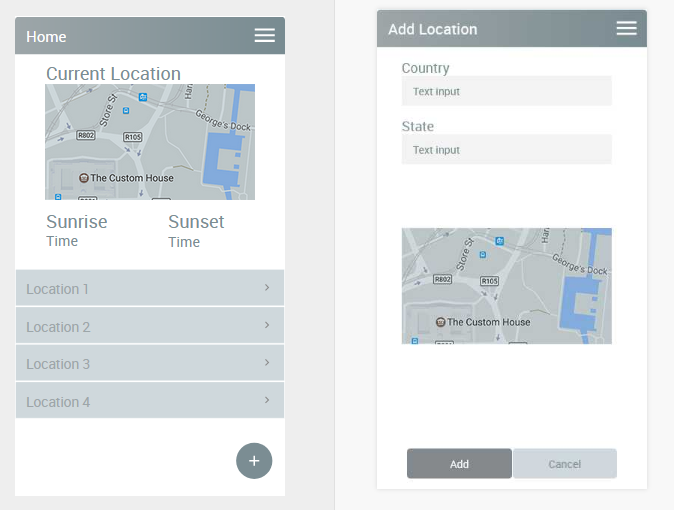
\includegraphics[scale=0.8]{images/screen1.png}
    \caption{The home and add location screens}
\end{figure}

\pagebreak

\begin{figure}[h]
    \centering
    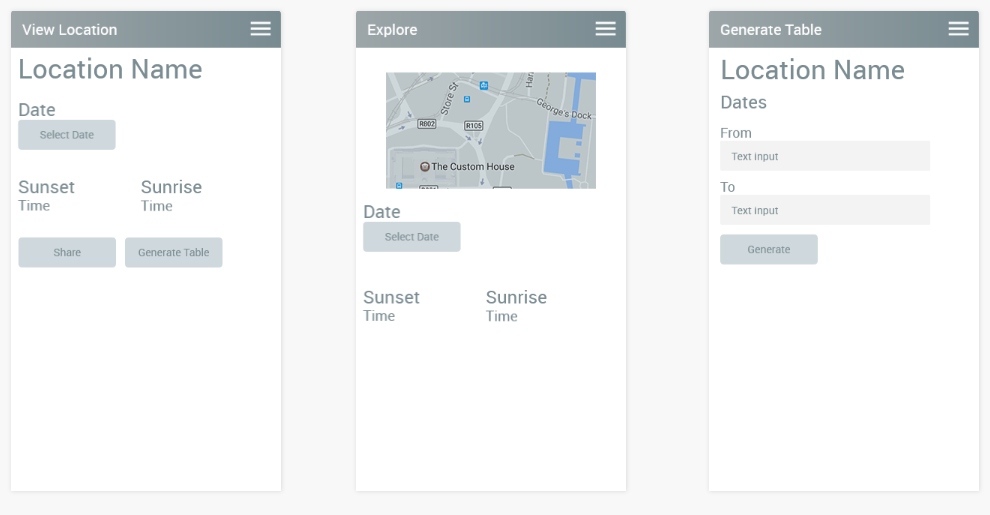
\includegraphics[scale=0.55]{images/screen2.png}
    \caption{The view location, explore, and generate table screens}
\end{figure}

\pagebreak

\section*{Part 2}
\begin{itemize}
    \item As a stargazer, I want to find the time of the local sunrise, so that I can schedule viewing times with minimal sunlight
    \begin{itemize}
        \item User looks at home screen for information based on current location
    \end{itemize}
    \item As a photographer, I want to view the sunrise and sunset times for the next 7 days so I can capture these events on camera.
    \begin{itemize}
        \item User taps on saved location
        \item User taps generate table
        \item User enters time period they wish to check
        \item User taps generate button
    \end{itemize}
    \item As a traveller, I want to find the time of sunset for my holiday destination, so that I can plan my holiday events in advance dinner with a great view
    \begin{itemize}
        \item User taps plus button
        \item User enters location information
        \item User taps location on home screen
    \end{itemize}
    \item As a traveller, I want to share the sunset time with my partner, so that I can organize a dinner with a great view
    \begin{itemize}
        \item User taps on saved location
        \item User taps generate table
        \item User taps generate
    \end{itemize}
\end{itemize}

\end{document}
